\documentclass[]{book}
\usepackage{lmodern}
\usepackage{amssymb,amsmath}
\usepackage{ifxetex,ifluatex}
\usepackage{fixltx2e} % provides \textsubscript
\ifnum 0\ifxetex 1\fi\ifluatex 1\fi=0 % if pdftex
  \usepackage[T1]{fontenc}
  \usepackage[utf8]{inputenc}
\else % if luatex or xelatex
  \ifxetex
    \usepackage{mathspec}
  \else
    \usepackage{fontspec}
  \fi
  \defaultfontfeatures{Ligatures=TeX,Scale=MatchLowercase}
\fi
% use upquote if available, for straight quotes in verbatim environments
\IfFileExists{upquote.sty}{\usepackage{upquote}}{}
% use microtype if available
\IfFileExists{microtype.sty}{%
\usepackage{microtype}
\UseMicrotypeSet[protrusion]{basicmath} % disable protrusion for tt fonts
}{}
\usepackage[margin=1in]{geometry}
\usepackage{hyperref}
\hypersetup{unicode=true,
            pdftitle={Cryptocurrency Research},
            pdfauthor={J.W.Biggs},
            pdfborder={0 0 0},
            breaklinks=true}
\urlstyle{same}  % don't use monospace font for urls
\usepackage{natbib}
\bibliographystyle{apalike}
\usepackage{color}
\usepackage{fancyvrb}
\newcommand{\VerbBar}{|}
\newcommand{\VERB}{\Verb[commandchars=\\\{\}]}
\DefineVerbatimEnvironment{Highlighting}{Verbatim}{commandchars=\\\{\}}
% Add ',fontsize=\small' for more characters per line
\usepackage{framed}
\definecolor{shadecolor}{RGB}{248,248,248}
\newenvironment{Shaded}{\begin{snugshade}}{\end{snugshade}}
\newcommand{\KeywordTok}[1]{\textcolor[rgb]{0.13,0.29,0.53}{\textbf{{#1}}}}
\newcommand{\DataTypeTok}[1]{\textcolor[rgb]{0.13,0.29,0.53}{{#1}}}
\newcommand{\DecValTok}[1]{\textcolor[rgb]{0.00,0.00,0.81}{{#1}}}
\newcommand{\BaseNTok}[1]{\textcolor[rgb]{0.00,0.00,0.81}{{#1}}}
\newcommand{\FloatTok}[1]{\textcolor[rgb]{0.00,0.00,0.81}{{#1}}}
\newcommand{\ConstantTok}[1]{\textcolor[rgb]{0.00,0.00,0.00}{{#1}}}
\newcommand{\CharTok}[1]{\textcolor[rgb]{0.31,0.60,0.02}{{#1}}}
\newcommand{\SpecialCharTok}[1]{\textcolor[rgb]{0.00,0.00,0.00}{{#1}}}
\newcommand{\StringTok}[1]{\textcolor[rgb]{0.31,0.60,0.02}{{#1}}}
\newcommand{\VerbatimStringTok}[1]{\textcolor[rgb]{0.31,0.60,0.02}{{#1}}}
\newcommand{\SpecialStringTok}[1]{\textcolor[rgb]{0.31,0.60,0.02}{{#1}}}
\newcommand{\ImportTok}[1]{{#1}}
\newcommand{\CommentTok}[1]{\textcolor[rgb]{0.56,0.35,0.01}{\textit{{#1}}}}
\newcommand{\DocumentationTok}[1]{\textcolor[rgb]{0.56,0.35,0.01}{\textbf{\textit{{#1}}}}}
\newcommand{\AnnotationTok}[1]{\textcolor[rgb]{0.56,0.35,0.01}{\textbf{\textit{{#1}}}}}
\newcommand{\CommentVarTok}[1]{\textcolor[rgb]{0.56,0.35,0.01}{\textbf{\textit{{#1}}}}}
\newcommand{\OtherTok}[1]{\textcolor[rgb]{0.56,0.35,0.01}{{#1}}}
\newcommand{\FunctionTok}[1]{\textcolor[rgb]{0.00,0.00,0.00}{{#1}}}
\newcommand{\VariableTok}[1]{\textcolor[rgb]{0.00,0.00,0.00}{{#1}}}
\newcommand{\ControlFlowTok}[1]{\textcolor[rgb]{0.13,0.29,0.53}{\textbf{{#1}}}}
\newcommand{\OperatorTok}[1]{\textcolor[rgb]{0.81,0.36,0.00}{\textbf{{#1}}}}
\newcommand{\BuiltInTok}[1]{{#1}}
\newcommand{\ExtensionTok}[1]{{#1}}
\newcommand{\PreprocessorTok}[1]{\textcolor[rgb]{0.56,0.35,0.01}{\textit{{#1}}}}
\newcommand{\AttributeTok}[1]{\textcolor[rgb]{0.77,0.63,0.00}{{#1}}}
\newcommand{\RegionMarkerTok}[1]{{#1}}
\newcommand{\InformationTok}[1]{\textcolor[rgb]{0.56,0.35,0.01}{\textbf{\textit{{#1}}}}}
\newcommand{\WarningTok}[1]{\textcolor[rgb]{0.56,0.35,0.01}{\textbf{\textit{{#1}}}}}
\newcommand{\AlertTok}[1]{\textcolor[rgb]{0.94,0.16,0.16}{{#1}}}
\newcommand{\ErrorTok}[1]{\textcolor[rgb]{0.64,0.00,0.00}{\textbf{{#1}}}}
\newcommand{\NormalTok}[1]{{#1}}
\usepackage{longtable,booktabs}
\usepackage{graphicx,grffile}
\makeatletter
\def\maxwidth{\ifdim\Gin@nat@width>\linewidth\linewidth\else\Gin@nat@width\fi}
\def\maxheight{\ifdim\Gin@nat@height>\textheight\textheight\else\Gin@nat@height\fi}
\makeatother
% Scale images if necessary, so that they will not overflow the page
% margins by default, and it is still possible to overwrite the defaults
% using explicit options in \includegraphics[width, height, ...]{}
\setkeys{Gin}{width=\maxwidth,height=\maxheight,keepaspectratio}
\IfFileExists{parskip.sty}{%
\usepackage{parskip}
}{% else
\setlength{\parindent}{0pt}
\setlength{\parskip}{6pt plus 2pt minus 1pt}
}
\setlength{\emergencystretch}{3em}  % prevent overfull lines
\providecommand{\tightlist}{%
  \setlength{\itemsep}{0pt}\setlength{\parskip}{0pt}}
\setcounter{secnumdepth}{5}
% Redefines (sub)paragraphs to behave more like sections
\ifx\paragraph\undefined\else
\let\oldparagraph\paragraph
\renewcommand{\paragraph}[1]{\oldparagraph{#1}\mbox{}}
\fi
\ifx\subparagraph\undefined\else
\let\oldsubparagraph\subparagraph
\renewcommand{\subparagraph}[1]{\oldsubparagraph{#1}\mbox{}}
\fi

%%% Use protect on footnotes to avoid problems with footnotes in titles
\let\rmarkdownfootnote\footnote%
\def\footnote{\protect\rmarkdownfootnote}

%%% Change title format to be more compact
\usepackage{titling}

% Create subtitle command for use in maketitle
\newcommand{\subtitle}[1]{
  \posttitle{
    \begin{center}\large#1\end{center}
    }
}

\setlength{\droptitle}{-2em}
  \title{Cryptocurrency Research}
  \pretitle{\vspace{\droptitle}\centering\huge}
  \posttitle{\par}
  \author{J.W.Biggs}
  \preauthor{\centering\large\emph}
  \postauthor{\par}
  \predate{\centering\large\emph}
  \postdate{\par}
  \date{2018-05-06}

\usepackage{booktabs}
\usepackage{amsthm}
\makeatletter
\def\thm@space@setup{%
  \thm@preskip=8pt plus 2pt minus 4pt
  \thm@postskip=\thm@preskip
}
\makeatother

\usepackage{amsthm}
\newtheorem{theorem}{Theorem}[chapter]
\newtheorem{lemma}{Lemma}[chapter]
\newtheorem{corollary}{Corollary}[chapter]
\newtheorem{proposition}{Proposition}[chapter]
\newtheorem{conjecture}{Conjecture}[chapter]
\theoremstyle{definition}
\newtheorem{definition}{Definition}[chapter]
\theoremstyle{definition}
\newtheorem{example}{Example}[chapter]
\theoremstyle{definition}
\newtheorem{exercise}{Exercise}[chapter]
\theoremstyle{remark}
\newtheorem*{remark}{Remark}
\newtheorem*{solution}{Solution}
\begin{document}
\maketitle

{
\setcounter{tocdepth}{1}
\tableofcontents
}
\chapter{About}\label{about}

This is research I have conducted for personal use. Using the Rmarkdown
language has enabled me to piece together research neatly and also quite
quickly. The folder containing all of research is available on request.

\url{http://www.coinmarketcap.com}

Remember each Rmd file contains one and only one chapter, and a chapter
is defined by the first-level heading \texttt{\#}.

To compile this example to PDF, you need XeLaTeX. You are recommended to
install TinyTeX (which includes XeLaTeX):
\url{https://yihui.name/tinytex/}.

\chapter{Introduction}\label{intro}

You can label chapter and section titles using \texttt{\{\#label\}}
after them, e.g., we can reference Chapter \ref{intro}. If you do not
manually label them, there will be automatic labels anyway, e.g.,
Chapter \ref{methods}.

Figures and tables with captions will be placed in \texttt{figure} and
\texttt{table} environments, respectively.

to see if this changes intro here is a set of text.

\begin{Shaded}
\begin{Highlighting}[]
\KeywordTok{par}\NormalTok{(}\DataTypeTok{mar =} \KeywordTok{c}\NormalTok{(}\DecValTok{4}\NormalTok{, }\DecValTok{4}\NormalTok{, .}\DecValTok{1}\NormalTok{, .}\DecValTok{1}\NormalTok{))}
\KeywordTok{plot}\NormalTok{(pressure, }\DataTypeTok{type =} \StringTok{'b'}\NormalTok{, }\DataTypeTok{pch =} \DecValTok{19}\NormalTok{)}
\end{Highlighting}
\end{Shaded}

\begin{figure}

{\centering \includegraphics[width=0.8\linewidth]{Cryptocurrency_Research_files/figure-latex/nice-fig-1} 

}

\caption{Here is a nice figure!}\label{fig:nice-fig}
\end{figure}

Reference a figure by its code chunk label with the \texttt{fig:}
prefix, e.g., see Figure \ref{fig:nice-fig}. Similarly, you can
reference tables generated from \texttt{knitr::kable()}, e.g., see Table
\ref{tab:nice-tab}.

\begin{Shaded}
\begin{Highlighting}[]
\NormalTok{knitr::}\KeywordTok{kable}\NormalTok{(}
  \KeywordTok{head}\NormalTok{(iris, }\DecValTok{20}\NormalTok{), }\DataTypeTok{caption =} \StringTok{'Here is a nice table!'}\NormalTok{,}
  \DataTypeTok{booktabs =} \OtherTok{TRUE}
\NormalTok{)}
\end{Highlighting}
\end{Shaded}

\begin{table}

\caption{\label{tab:nice-tab}Here is a nice table!}
\centering
\begin{tabular}[t]{rrrrl}
\toprule
Sepal.Length & Sepal.Width & Petal.Length & Petal.Width & Species\\
\midrule
5.1 & 3.5 & 1.4 & 0.2 & setosa\\
4.9 & 3.0 & 1.4 & 0.2 & setosa\\
4.7 & 3.2 & 1.3 & 0.2 & setosa\\
4.6 & 3.1 & 1.5 & 0.2 & setosa\\
5.0 & 3.6 & 1.4 & 0.2 & setosa\\
\addlinespace
5.4 & 3.9 & 1.7 & 0.4 & setosa\\
4.6 & 3.4 & 1.4 & 0.3 & setosa\\
5.0 & 3.4 & 1.5 & 0.2 & setosa\\
4.4 & 2.9 & 1.4 & 0.2 & setosa\\
4.9 & 3.1 & 1.5 & 0.1 & setosa\\
\addlinespace
5.4 & 3.7 & 1.5 & 0.2 & setosa\\
4.8 & 3.4 & 1.6 & 0.2 & setosa\\
4.8 & 3.0 & 1.4 & 0.1 & setosa\\
4.3 & 3.0 & 1.1 & 0.1 & setosa\\
5.8 & 4.0 & 1.2 & 0.2 & setosa\\
\addlinespace
5.7 & 4.4 & 1.5 & 0.4 & setosa\\
5.4 & 3.9 & 1.3 & 0.4 & setosa\\
5.1 & 3.5 & 1.4 & 0.3 & setosa\\
5.7 & 3.8 & 1.7 & 0.3 & setosa\\
5.1 & 3.8 & 1.5 & 0.3 & setosa\\
\bottomrule
\end{tabular}
\end{table}

You can write citations, too. For example, we are using the
\textbf{bookdown} package \citep{R-bookdown} in this sample book, which
was built on top of R Markdown and \textbf{knitr} \citep{xie2015}.

\chapter{Literature}\label{literature}

Here is a review of existing methods.

\chapter{What is Digital Currency?}\label{what-is-digital-currency}

\section{Let's Get the terms Right}\label{lets-get-the-terms-right}

If you were to look up the term `cryptocurrency' you would get something
like or similar to the following definition: A digital or virtual
currency, that uses cryptographic encryption techniques to generate
units of the currency and verify transactions. It is important to add
however, that many use the term `digital currency' interchangeably with
`cryptocurrency'. Why it is important to make a distinction will be
covered later, but first let's substantiate the claim that the terms are
used interchangeably.

If you were to type `digital currency' into Google's news search you
would most likely receive articles about cryptocurrency and in
particular Bitcoin. As can be seen below. I've taken the first 20
articles from google news (week of 20th feb), and taken their text using
it in a word matrix. As can be seen from the matrix below `Bitcoin' is
the most popular topic associated with the term `digital'.

\begin{figure}[htbp]
\centering
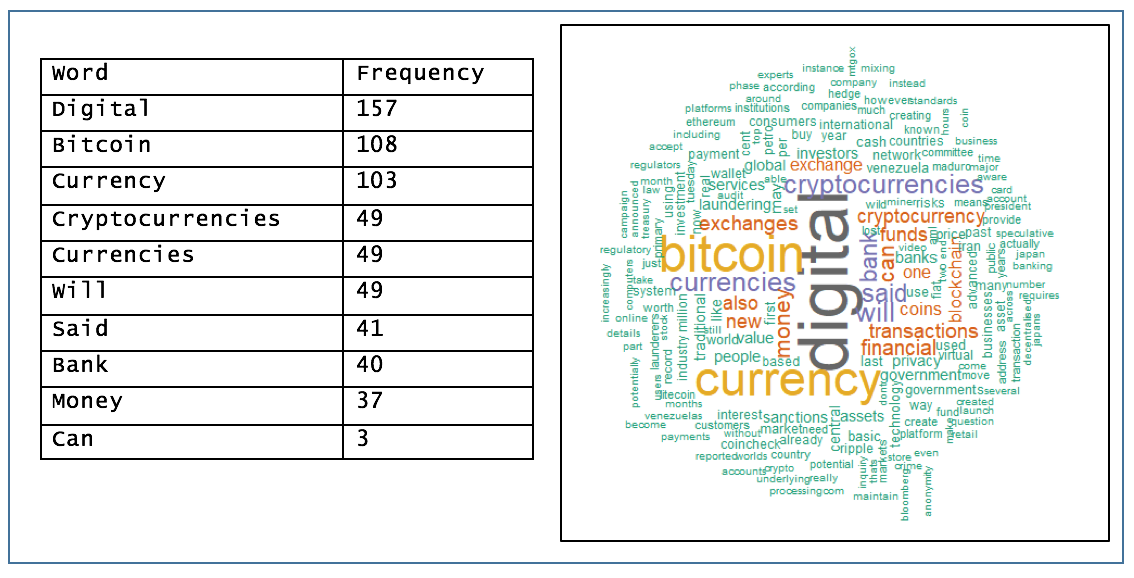
\includegraphics{~/Desktop/Everything/R/Working Directory/Cryptocurrency book/pictures/Example.png}
\caption{}
\end{figure}

\section{Advancing a clear
definition}\label{advancing-a-clear-definition}

It would be very easy for anyone interested in digital currency right
now to focus on Bitcoin which is actually only a tiny element of what is
covered by the term `digital currency'. To define cryptocurrency well we
first need to understand what separates it from other digital
currencies.

Digital Currency as a broad term can contain anything that represents
value in a digital manner. Digital currency can contain firstly what we
would call electronic `money', money that is simply a digital
representation of government issued fiat currency. Fiat currency is
government backed, so whilst it has no intrinsic value, i.e it is not
tied to a commodity such as gold, it is considered legal tender.

Digital currency can also cover virtual currency -- electronic currency
that it is not considered legal tender. Virtual currencies are
controlled and created by their developers, with value being appreciated
in a specific community. A prime example would be Nintendo points, users
can either earn units of currency or points by completing game
challenges or by exchanging fiat currency for them. Once bought,
Nintendo points are only useful in the Nintendo ecosphere and seldom
used elsewhere.

With the above understood, the final area of digital currency to examine
is Cryptocurrency -- a decentralised virtual currency. It is a virtual
currency because its units are not considered legal tender, but is
separate from other virtual currencies because its units are created and
handled without any overseer required.

The international monetary fund and the European bank have only recently
put together a taxonomy of digital currency. A visual representation of
how I have defined terms has been provided below.

\subsection{Taxonomy of Digital
Currency}\label{taxonomy-of-digital-currency}

\begin{figure}[htbp]
\centering
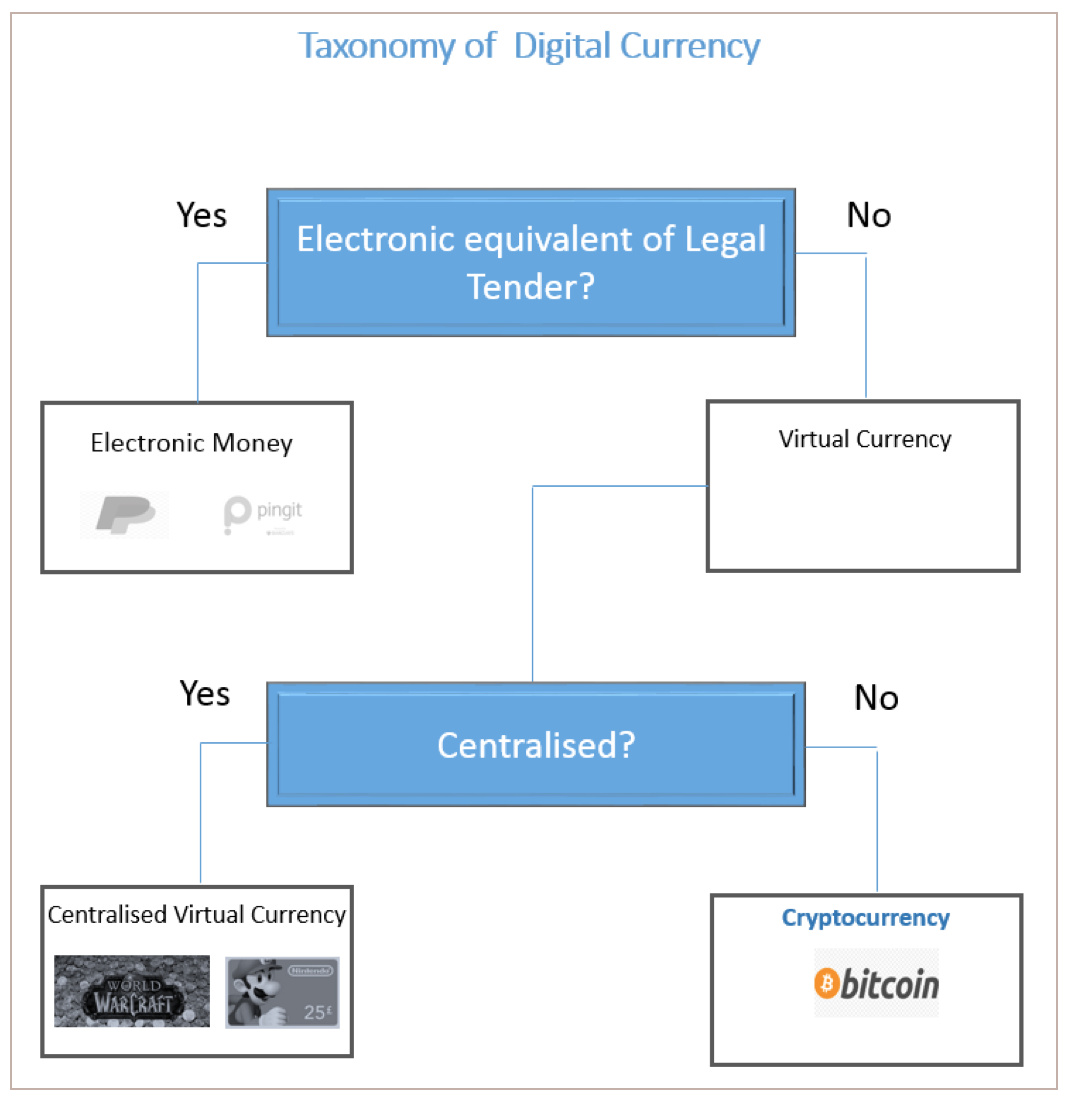
\includegraphics{~/Desktop/Everything/R/Working Directory/Cryptocurrency book/pictures/Taxonomy.png}
\caption{}
\end{figure}

\subsection{Digital currency before
Bitcoin}\label{digital-currency-before-bitcoin}

If we understand that Digital currency is just an electronic
representation of any asset, it is useful to point out and understand
that digital currency can be traced back to the 1960s. Here are the main
highlights I've found from research:

\begin{figure}[htbp]
\centering
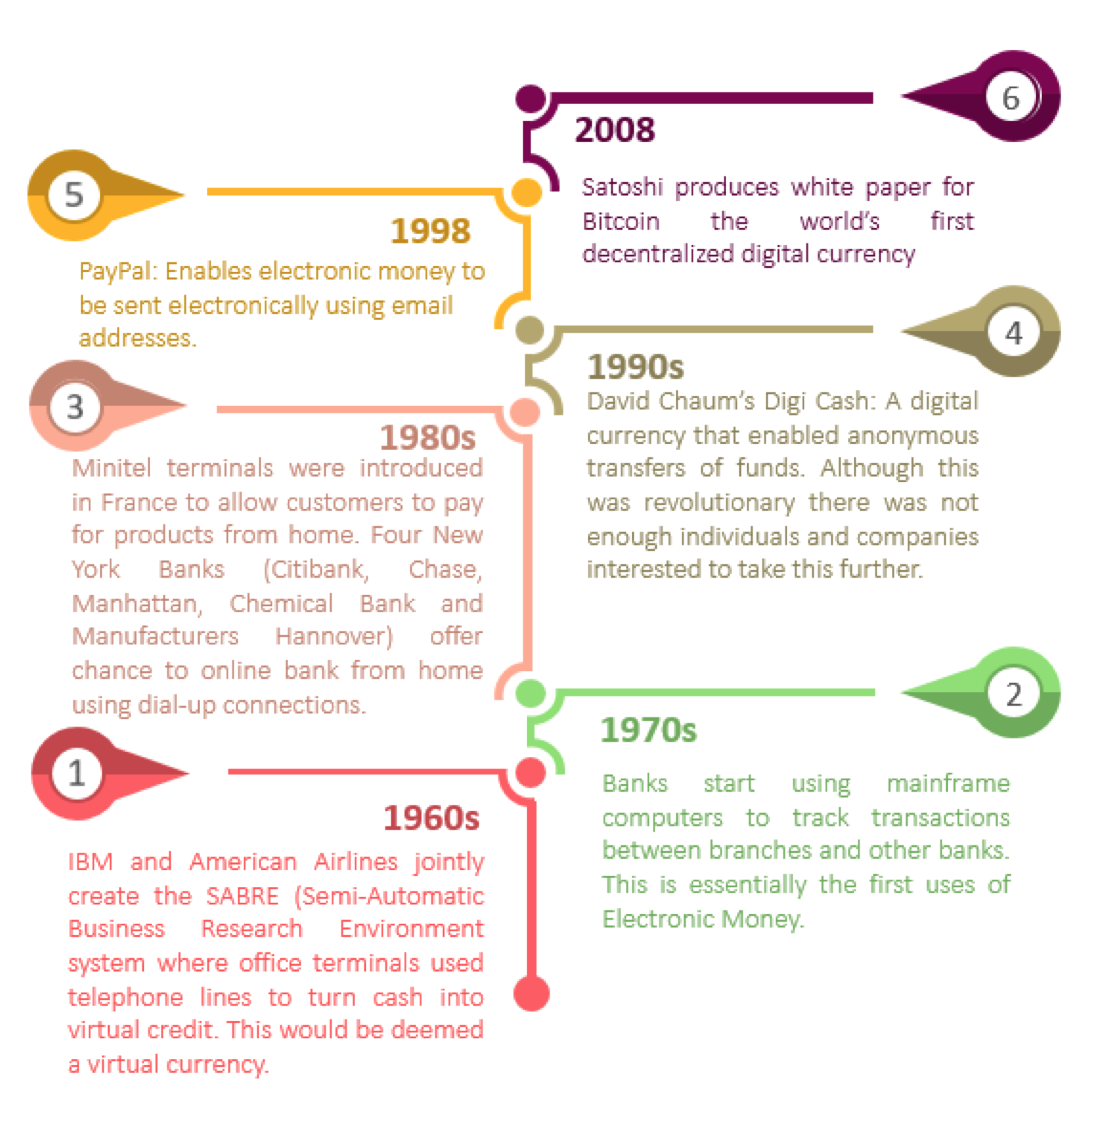
\includegraphics{~/Desktop/Everything/R/Working Directory/Cryptocurrency book/pictures/Timeline.png}
\caption{}
\end{figure}

\chapter{How does Cryptocurrency
Funtion?}\label{how-does-cryptocurrency-funtion}

\subsection{\texorpdfstring{Achieving `distributed
consensus'}{Achieving distributed consensus}}\label{achieving-distributed-consensus}

Bitcoin was the first digital currency that functioned without a central
mediator. Before Bitcoin came about there was no way to achieve
distributed consensus without a centralised actor. Distributed consensus
simply means a large pool of people who are geographically segregated
agreeing on something. The way that Bitcoin solved the issues of trust
that made a decentralised currency impossible to achieve was the
invention of the Blockchain.

\subsection{What was Bitcoin's
Blockchain?}\label{what-was-bitcoins-blockchain}

Bitcoin's Blockchain is essentially applied three main cryptographic
concepts to a single distributed ledger (an open ledger everyone has
access to): Digital Signatures, Merkle Trees, and the cryptographic
concept of Proof-of-Work.

\begin{figure}[htbp]
\centering
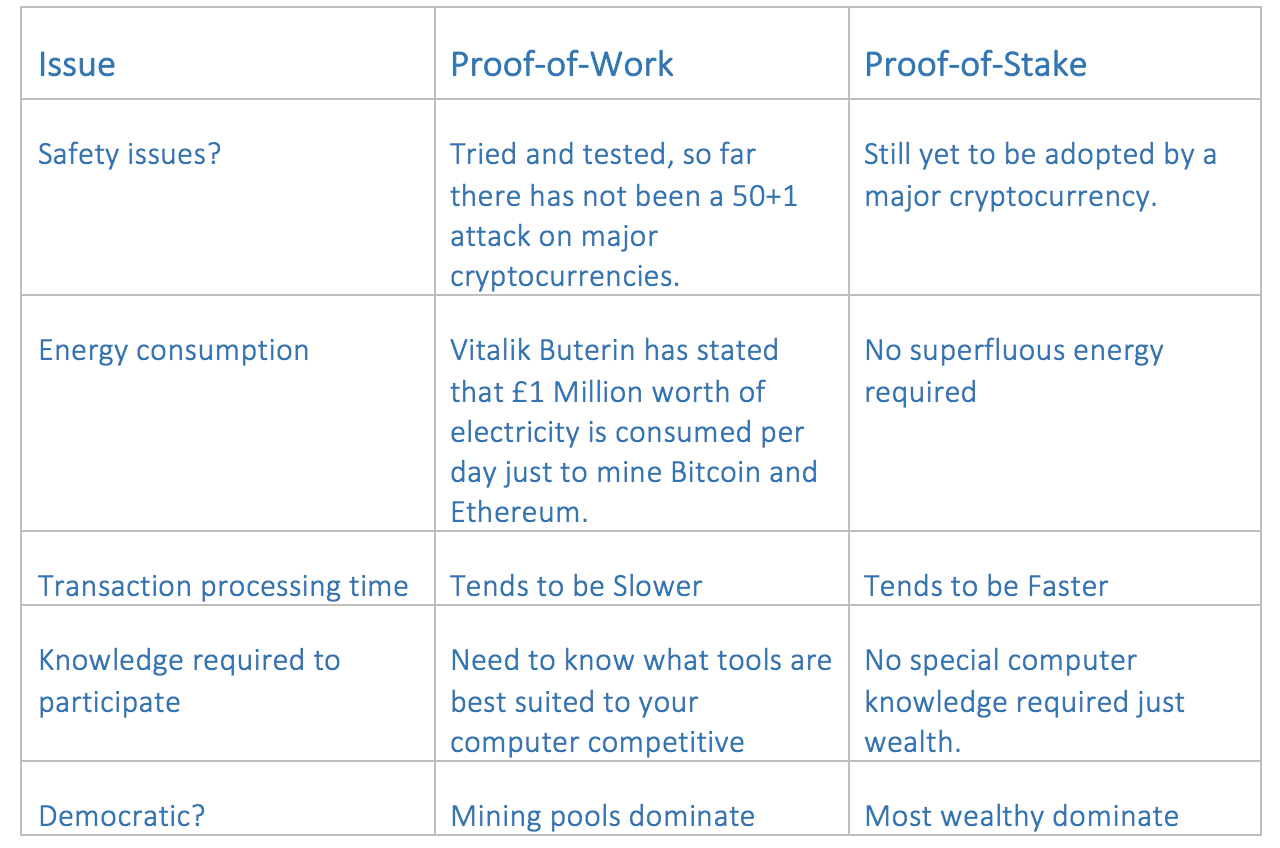
\includegraphics{~/Desktop/Everything/R/Working Directory/Cryptocurrency book/pictures/PoW_V_Pos.png}
\caption{}
\end{figure}

\subsection{Digital Signatures}\label{digital-signatures}

Digital signatures ensure that all transactions on the network are
authentic. Every transaction will be encrypted with the signing key can
only be decrypted with the verification key. Digital signatures are
applied so that every transaction has a unique signature that could only
be achieved with a private key. A useful to think of it, is when someone
makes a transaction to an address he/she essentially states that `I give
the right to spend this money to the person who owns the private key
corresponding to this address'. The person who has received this
transaction will in turn be able to spend the transaction by signing the
transaction using his private key. With this signature, he can prove
that he owns the key, without even disclosing it. Others can verify the
signature using the public key.''

\subsection{Merkle Trees}\label{merkle-trees}

Merkle trees provide a way to chain together groups of authenticated
transactions. Merkle trees ensure this by utilizing the technique of
hashing. Hashing is the transformation of string of characters into a
usually shorter fixed-length value or key that represents the original
string. Each block is chained to the preceding block by containing a
hash that could only be generated using the previous block's hash. For
this reason, Merkle trees are often also referred to as Hash trees. Here
is a useful video tutorial of this.

\begin{figure}[htbp]
\centering
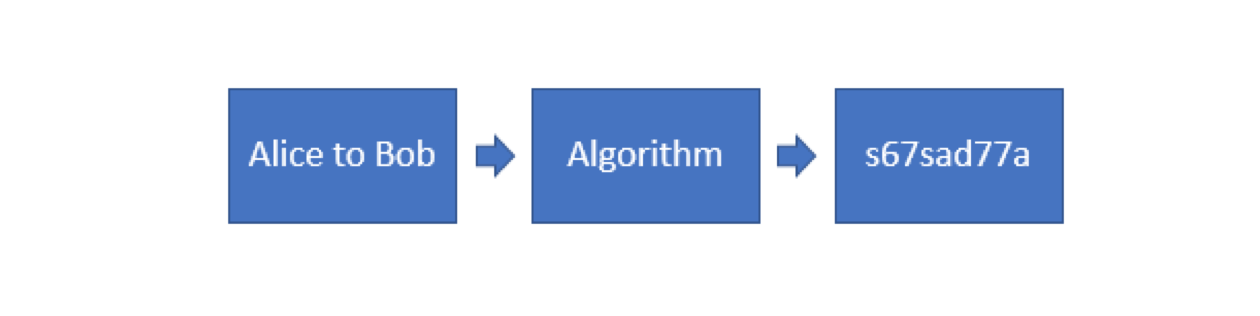
\includegraphics{~/Desktop/Everything/R/Working Directory/Cryptocurrency book/pictures/hashing.png}
\caption{Hashing explained}
\end{figure}

We can see that the smallest change in the message will drastically
alter the resulting hash. Merkle trees work by using hashes to create a
chain, where a block of data can only be added by using the previous
hash. If one block is changed then the rest of the blocks will be
changed. This is visually represented below. Numbers have been used
instead of actual hashes for clarity.

\begin{figure}[htbp]
\centering
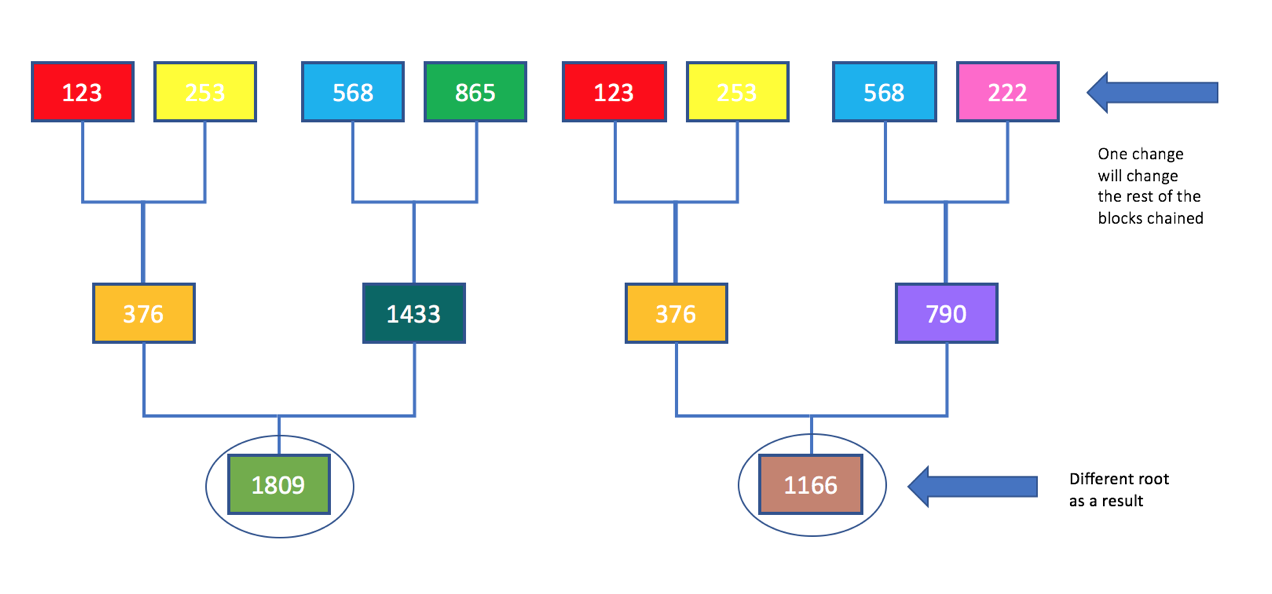
\includegraphics{~/Desktop/Everything/R/Working Directory/Cryptocurrency book/pictures/merkle_treee.png}
\caption{How Merkle trees function}
\end{figure}

\subsection{Proof-of-Work concept}\label{proof-of-work-concept}

The first two cryptographic techniques have ensured that every
transaction requested to added to the ledger is authentic and there is a
way to order the transactions into blocks. However, if the Bitcoin
creators left things here it would still be chaos.

There wouldn't be a way of agreeing which chain of blocks to choose to
summarize all transactions, there would lots of different versions
emerging. This is where proof-of-work comes in. Proof-of-work ensures
that each block added takes time to ensure that there is order and one
single chain of blocks. Users dedicating time to process transactions
they are rewarded units of currency.

What is exactly this proof-of-work? Essentially for each block to be
added to the chain it needs to undergo a validation process that
involves solving a puzzle. Each block starts with a default hash, this
is the block is put through a function that turns it into a set string
of unintelligible data as explained earlier. Users wishing to earn the
Bitcoin reward need to add other characters to the block until the
resulting hash starts in a certain number of zeros (currently 18). This
difficulty (more zeros required) is enhanced every time 2016 blocks are
added to the chain. The diagram below shows that with just one character
change.

\begin{figure}[htbp]
\centering
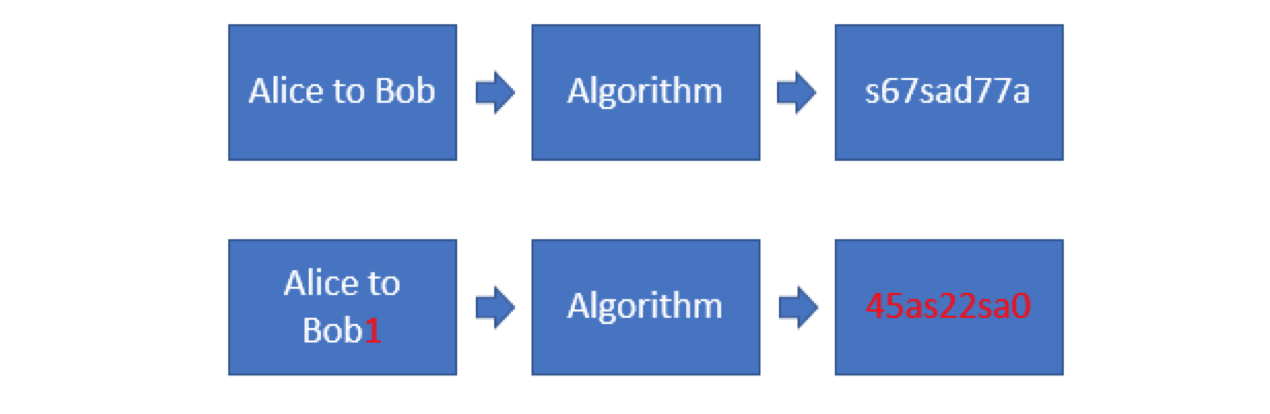
\includegraphics{~/Desktop/Everything/R/Working Directory/Cryptocurrency book/pictures/Proof_of_work.png}
\caption{In this instance we can see that just one change has
drastically altered the hash}
\end{figure}

\subsection{Alternative mechanisms to achieve distributed consensus:
Proof-of-stake}\label{alternative-mechanisms-to-achieve-distributed-consensus-proof-of-stake}

Proof work functions in a way that the more computational power you have
the more likely you are to add a block to the chain. Proof-of-Stake
functions in a way that the more wealth you stake towards the effort of
adding blocks to the chain the more likely you are to win the block
reward. In proof of work you will win a certain amount for instance 12.5
Bitcoin or 6 Ether. In proof-of-stake you will tend to win transaction
fees. In the visual scenario below we can see that Alice would have the
best chance of winning the block reward as see has largest proportion of
cryptocurrency.

\begin{figure}[htbp]
\centering
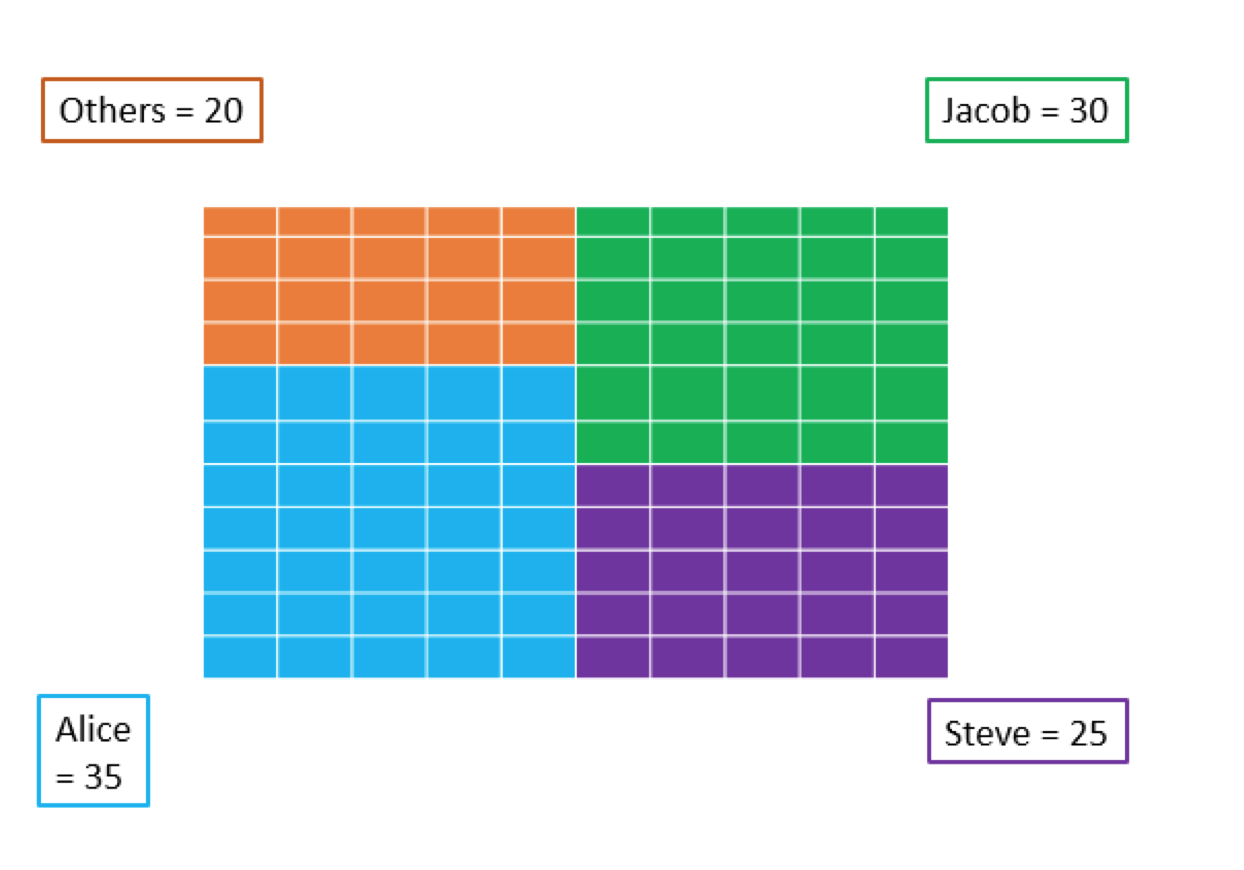
\includegraphics{~/Desktop/Everything/R/Working Directory/Cryptocurrency book/pictures/Proof_of_stake.png}
\caption{Proof of stake explained in a very simple visual manner}
\end{figure}

\subsection{Proof-of-Stake versus Proof-of-Work
Summarised}\label{proof-of-stake-versus-proof-of-work-summarised}

\begin{figure}[htbp]
\centering
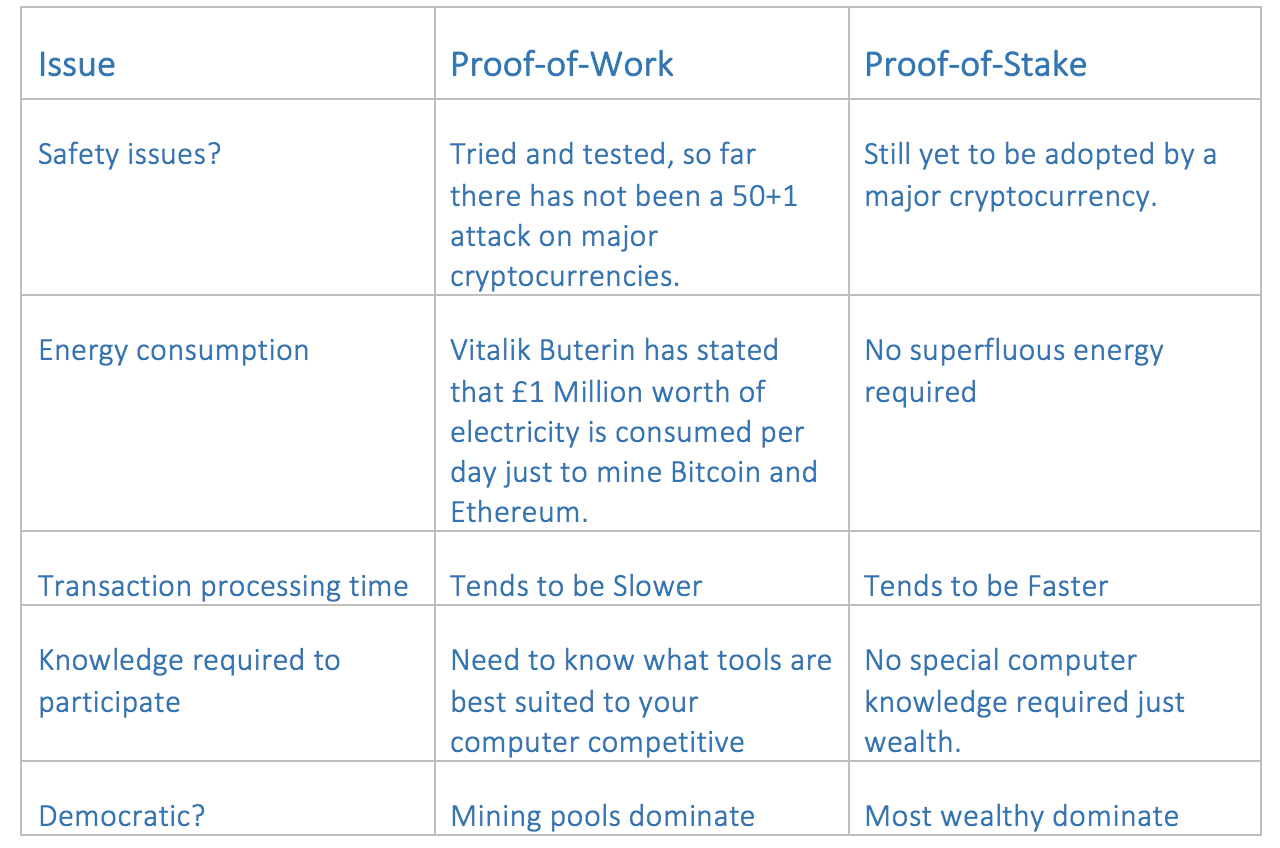
\includegraphics{~/Desktop/Everything/R/Working Directory/Cryptocurrency book/pictures/PoW_V_Pos.png}
\caption{Proof of stake explained in a very simple visual manner}
\end{figure}

\subsection{A Bitcoin transaction}\label{a-bitcoin-transaction}

If the above seems to technical here demonstration of transaction using
Bitcoin where technical terms have been taken out. It shows how Alice
would go about transferring Bitcoin to Bob.

\begin{figure}[htbp]
\centering
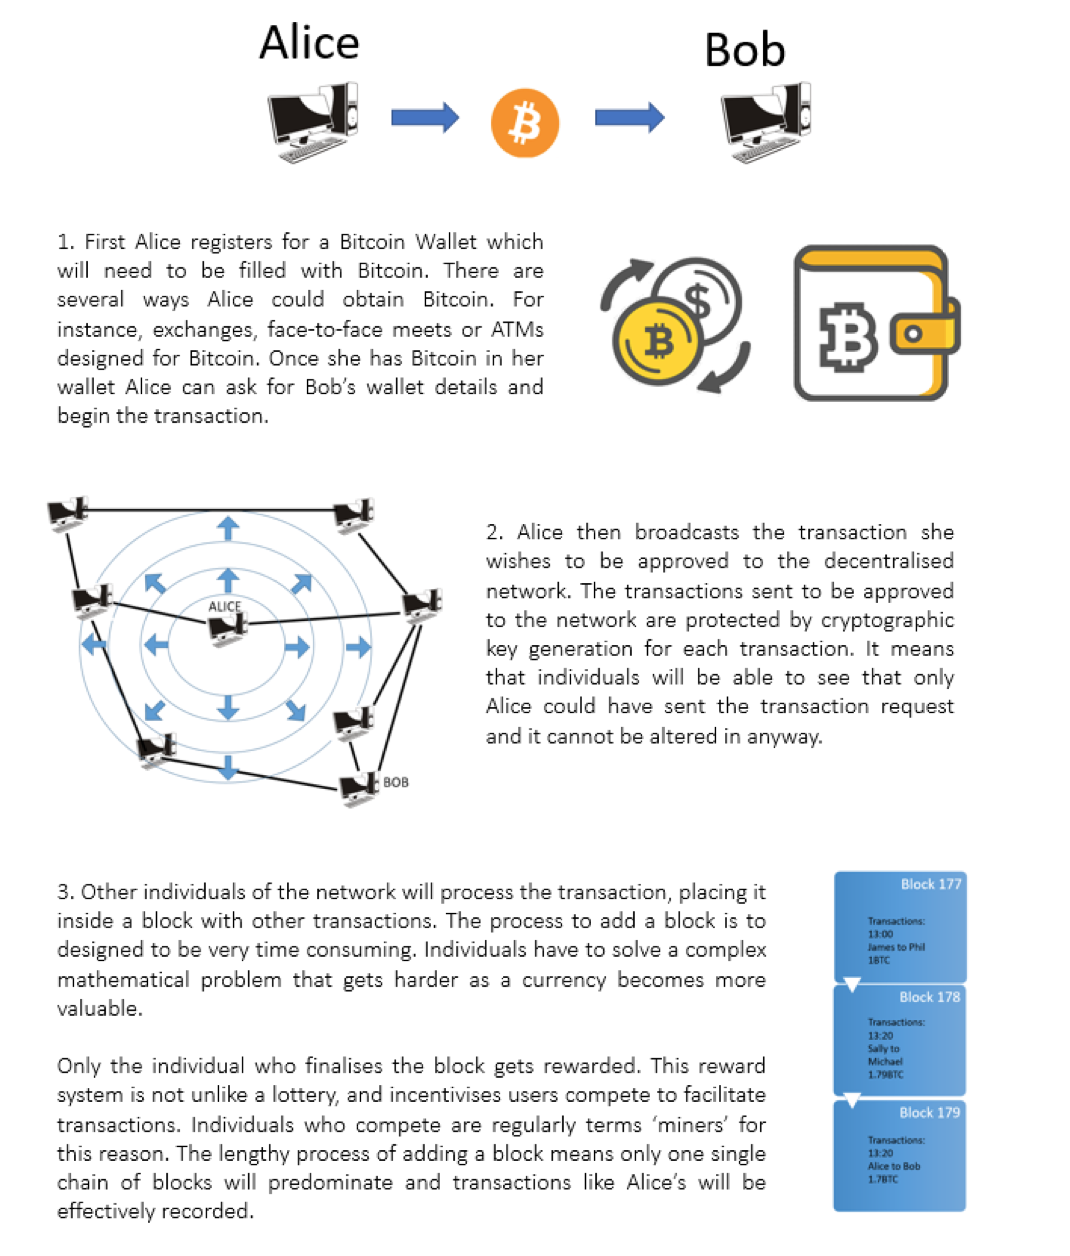
\includegraphics{~/Desktop/Everything/R/Working Directory/Cryptocurrency book/pictures/transaction.png}
\caption{Original image available upon request}
\end{figure}

\chapter{How do I obtain
Cryptocurrency?}\label{how-do-i-obtain-cryptocurrency}

There are a number of ways to obtain cryptocurrency. This chapter will
exemplify how an individual in the United Kingdom would obatin Bitcoin.

\section{Exchanges}\label{exchanges}

By far the easiest method to obtain cryptocurrency is by going through
an online exchange. Exchanges essentially allow individuals to exchange
fiat currency such as Great British Pounds or US Dollars into
Cryptocurrencies such as Bitcoin. Some Exchanges also allow individuals
to exchange cryptocurrencies for other cryptocurrencies. For instance,
Trading the most popular cryptocurrency Bitcoin for the second most
popular cryptocurrency Ethereum.

There are currently 130 Cryptocurrency Exchanges on the World Wide Web.
If we look at trades by minute the US based Coinbase exchange processed
the most trades by minute (22\% of total cryptocurrency trades per
minute). CEX an exchange based in London has made the top ten with 3\%
of trade made per minute going being processed with its services.

\begin{figure}[htbp]
\centering
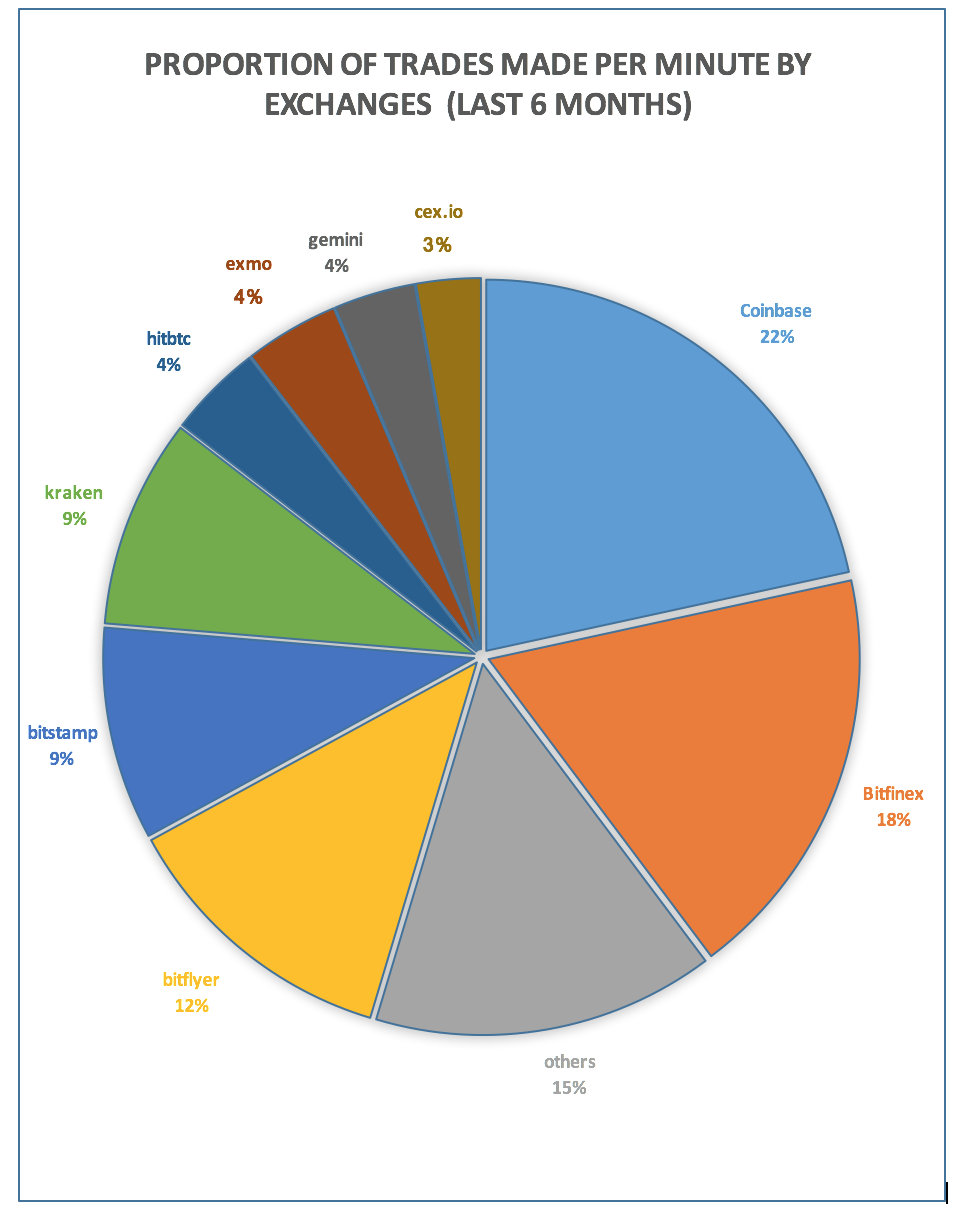
\includegraphics{~/Desktop/Everything/R/Working Directory/Cryptocurrency book/pictures/Exchanges.png}
\caption{The data for this was downloaded during February 2018}
\end{figure}

\section{Bitcoin ATMs}\label{bitcoin-atms}

A popular yet less common alternative to buying cryptocurrency is
through designated cryptocurrency automatic teller machines (ATMs).
There are a total of 103 cryptocurrency ATMS in the United Kingdom.77
ATMS of which are in London, 6 in Birmingham 20 in other cities with
just a few ATMS each.

\section{Bitcoin Meetups}\label{bitcoin-meetups}

Another way to get hold of cryptocurrency is to go to meetups where
cryptocurrency can be bought from individuals in person. For instance,
on meetup.com an individual could search for events held in their area
or nearby that facilitates a meetup for trades. Websites like
localbit.com also allow for individuals to buy and sell Bitcoin in
person. Individuals can list how much they are willing to sell and their
preferred method of payment.

\section{Mining for Bitcoin}\label{mining-for-bitcoin}

Mining is the process by which individuals on a cryptocurrency network
work to process cryptocurrency transactions. They are rewarded with
cryptocurrency for their efforts. Popular cryptocurrencies like Bitcoin
and Ethereum would be extremely difficult for a sole individual to
process as they are competing against a huge amount of computer power.

In fact some have estimated that mining for Bitcoin uses over 42TWh of
electricity in a year, which places its energy consumption higher than
New Zealand and Hungary. This said, mining can still be accomplished by
an individual by joining a mining pool -- a group of users combining
their computing power and sharing the proceeds if they win the reward of
processing a block of transactions.

\begin{figure}[htbp]
\centering
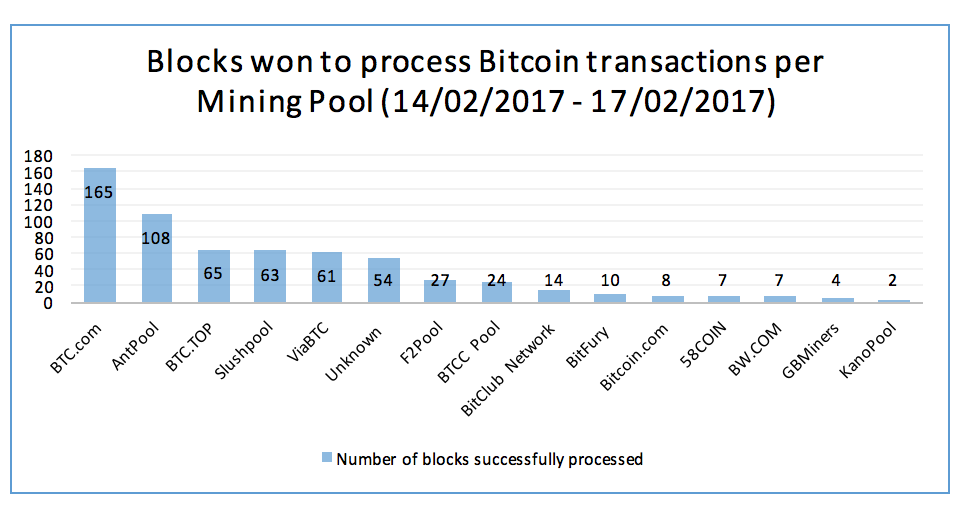
\includegraphics{~/Desktop/Everything/R/Working Directory/Cryptocurrency book/pictures/Mining_pools.png}
\caption{As above, please note data for this was downloaded in February}
\end{figure}

\chapter{Alternative
Cryptocurrencies}\label{alternative-cryptocurrencies}

As Bitcoin's source code is openly available, it means developers easily
build on it to create their own alternative cryptocurrencies or
`altcoins'. Many popular cryptocurrencies can be traced back to a major
cryptocurrency before. For instance, the cryptocurrency Dogecoin, was a
variant of Litecoin, which was a variant of Bitcoin.

\begin{figure}[htbp]
\centering

\includegraphics{~/Desktop/Everything/R/Working Directory/Cryptocurrency book/pictures/Lineage.png}
\caption{Litecoin changed adaption rates of Bitcoin, and Dogecoin of
Litecoin}
\end{figure}

If we analyze the very first altcoins we can see that there were only
small changes made to Bitcoin's original source code. Altcoins tended to
differentiate in a few aspects. Firstly, the amount of coins that could
be produced, the speed at which transactions were processed and the
reward given to those facilitating transactions. Below is a summary of
the first altcoins to be produced. Most are directly linked, with little
in the way of major differences.

\section{Altcoins from 2008 - 2012}\label{altcoins-from-2008---2012}

\begin{figure}[htbp]
\centering
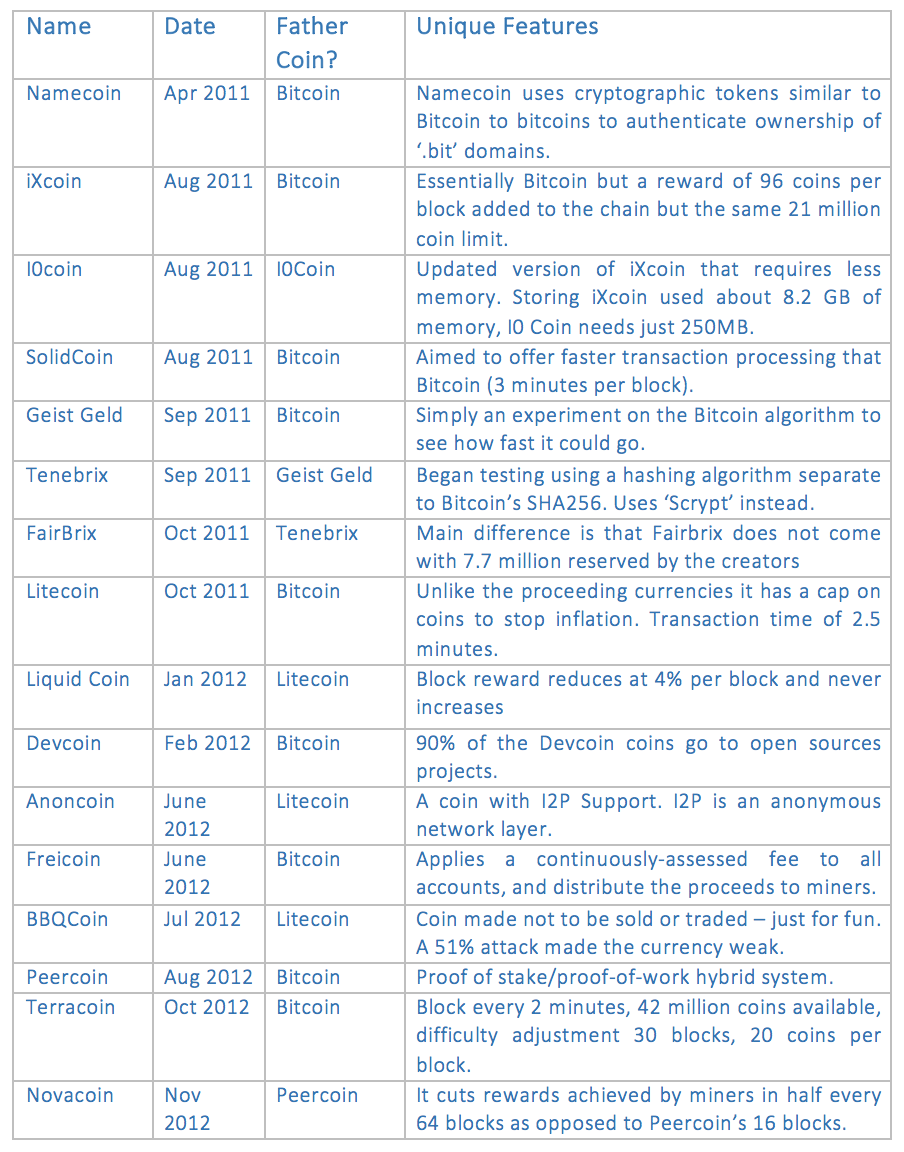
\includegraphics{~/Desktop/Everything/R/Working Directory/Cryptocurrency book/pictures/Altcoin.png}
\caption{It was mainly adoption rates that distinguished altcoins from
2008 to 2012}
\end{figure}

There are now thousands of cryptocurrencies listed on websites like
coinmarketcap.com. What has caused this explosion? For one as the
cryptocurrency ecosphere is dedicated to open source development
competent developers now have a host of other cryptocurrencies to build
on. Secondly, cryptocurrencies like Ethereum make it relatively easy to
create applications and altcoin on top of its blockchain. As of March
(28th) 2018 there are currently 1591 total cryptocurrencies listed on
www.coinmarketcap.com website.

\begin{figure}[htbp]
\centering
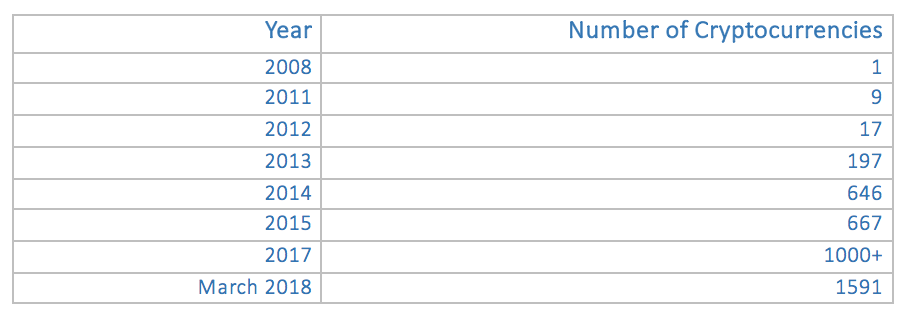
\includegraphics{~/Desktop/Everything/R/Working Directory/Cryptocurrency book/pictures/March_table.png}
\caption{The amount of cryptocurrencies has exploded since 2008}
\end{figure}

\section{Which Altcoin Currently
Predominate?}\label{which-altcoin-currently-predominate}

Here is the market capitalization at March 28th 2018 16:00.

\begin{figure}[htbp]
\centering
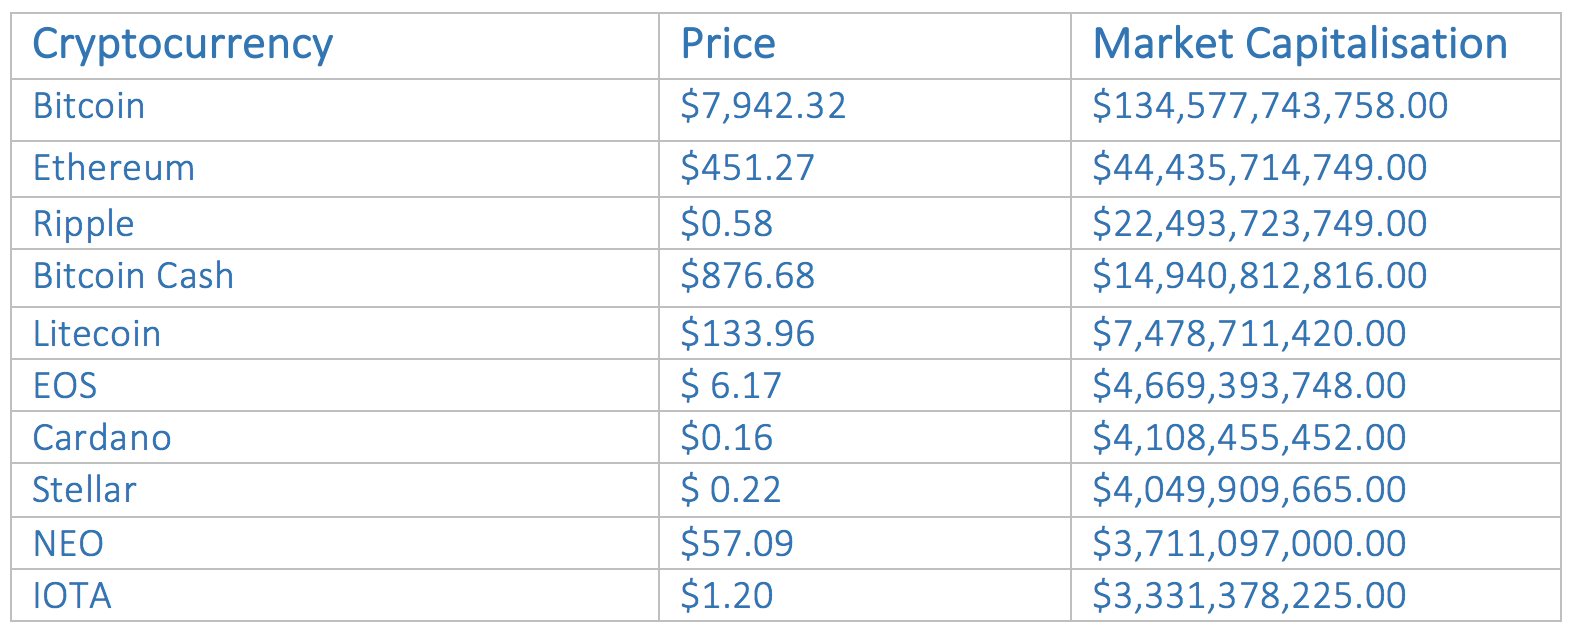
\includegraphics{~/Desktop/Everything/R/Working Directory/Cryptocurrency book/pictures/best_cryptos.png}
\caption{The amount of cryptocurrencies has exploded since 2008}
\end{figure}

The top ten cryptocurrencies differ from each other, but can be grouped
together in the qualities they share. Starting from Bitcoin as a core
cryptocurrency a quick summary is offered here:

\subsection{Bitcoin Cash and Litecoin}\label{bitcoin-cash-and-litecoin}

Bitcoin cash and Litecoin function in the same way as Bitcoin except
their adoption rates differ. Litecoin was designed so that transactions
could be processed quicker and has a different supply limited to Bitcoin
as covered earlier. Bitcoin Cash is essentially Bitcoin but with eight
times the scalability. It was a hard fork of Bitcoin where one camp
decided to create an entirely new cryptocurrency because of how to deal
with the scalability issues (current protocol cannot cope with the
amount of transactions being processed).

\subsection{Ripple and Stellar}\label{ripple-and-stellar}

Two of these, Ripple and Stellar, differ from above in that they are
designed as transaction networks. Most digital currencies are designed
to be stored unit of value however Ripple and Stellar are created to
digitalize regular fiat (national currency) transactions with their
tokens. Both digital currencies offer faster payment solutions by
utilizing blockchain technology. Ripple is suited towards banks and
stellar for individuals trading foreign currencies. Both have central
interference on what transactions are processed so it would be difficult
to call them pure `cryptocurrencies'.

\subsection{\texorpdfstring{`Second Generation'
Cryptocurrencies}{Second Generation Cryptocurrencies}}\label{second-generation-cryptocurrencies}

The rest of the cryptocurrencies in the top ten can be considered much
more than a store of value or a payments processing service. Ethereum,
EOS, Cardano, NEO and IOTA all offer the ability for users to build on
top of them. Instead of just being a currency, they have been designed
to be built on top of. Ethereum was the first cryptocurrency designed
specifically to make building applications on top of a blockchain easy.
The others above essentially enable individuals to do the same but
differ from Ethereum in several aspects. Here is a good article
explaining the pros and cons of each decentralized platform

\chapter{Final Words}\label{final-words}

We have finished a nice book.

\chapter{Second Generation
Cryptocurrencies}\label{second-generation-cryptocurrencies-1}

Cryptocurrencies that enable smart contracts and decentralized
applications to easily be constructed are often called `second
generation' cryptocurrencies. Whilst there were a few smart contracts
built on top of Bitcoin such Mastercoin (now Omni) and Coloured Coins
these were difficult to build. Ethereum made smart contracts much easier
to build by constructing a completely unique language that could be
easily integrated with its purpose-built platform. Essentially Ethereum
made it easily possible to add updated details of ongoing smart
contracts or add new smart contract details into blocks with
transactions simultaneously being processed on the network. Ethereum is
far by most commonly used platform to build a variety of different
decentralized applications.

\section{What are Smart Contracts}\label{what-are-smart-contracts}

A smart contract is a piece of code that implements arbitrary rules. A
useful way of thinking about smart contracts is just to realise that
smart contracts are essentially the same as contracts - with the
difference that they will automatically execute any actions that parties
involved have agreed.

Let's use Vitalik Buterin's (creator of Ethereum) scenario to explain
what a smart contract is. Futhermore lets say the scenario is that A
wants to pay B \$500 to build a website

\begin{enumerate}
\def\labelenumi{\arabic{enumi}.}
\tightlist
\item
  Contract agreement: A puts \$500 into the contract, funds are locked.
\item
  B finishes website and sends a message to the contract asking to
  unlock the funds
\item
  If A agrees funds are released.
\item
  If B decides to not finish the website B can quit by sending a message
  to relinquish funds.
\item
  If A and B disagree it will be up to a defined judge (both A and B
  agree on who this is at the start) to decide.
\end{enumerate}

In Vitalik's own words: The ``basic concept {[}of a smart contract{]} is
if you have some new kind of application what you would do is write the
rules of your application in a piece of code\ldots{} Take this piece of
code you would call this a contract''. Once you've uploaded this to the
blockchain you have a special type of account that is essentially
controlled by the code you have written. The moment you send one ether
to that account you relinquish control of that account and no one
controls it anymore -- it is essentially a robot that sits on top of the
blockchain.

\section{What are Decentralised
Applications}\label{what-are-decentralised-applications}

Let's start with what an application is. An application is piece of
software designed for a specific purpose. Microsoft PowerPoint for
instance is an application that allows you to create slideshows for
presentations. A decentralized application is just an application that
does not have a no single point of information to run the application.
For instance, a web App like Facebook will have a central server to
connect to. Whereas any app built on Ethereum's blockchain will be run
through the smart contracts designed to run it. There is no agreed
definite definition of what a DApp is but there is a broad consensus on
what the three main characteristics are for DApps involving monetary
value.

Firstly a DApp tends to be Open Source: A DApp is characterized by its
transparent nature. Open source means that anyone can see the code that
was used to build the DApp. Secondly a DApp has Internal Currency or
Tokens: Because decentralised apps are open sourced charging users for
the service would be fruitless. The answer is to allocate scare
resources in the network by using a scarce token. Owners of scare
resources get paid in unit's native to the DApp. As the DApp becomes
bigger and more used these scarce resources become more valuable.
Thirdly a DApp will have a Mechanism to achieve decentralized consensus:
As there is no single entity controlling the application, distributed
consensus needs to be achieved without trust. For this reason, Bitcoin
can be considered one of the first monetary DApps as well as the first
cryptocurrency.

\section{DApp development: the current
picture}\label{dapp-development-the-current-picture}

As mentioned earlier the main reason that many DApps are built with
Ethereum is because it was the first to implement a unique code to
enable widespread adoption of them. With Smart Contracts, Ethereum has
made it easy for DApp developers to create their own tokens to fuel
their DApps. The ERC20 token standard developed in 2015 defines a common
list of rules that an Ethereum token has to implement. Ethereum's
protocol has become very popular with crowdfunding companies. Ethereum
even provides its own guide that shows you how to use smart contracts to
create a token -- mentioning at the end that they are very useful for
crowd sales www.ethereum.org/token.

\subsection{How many tokens are associated with
Ethereum?}\label{how-many-tokens-are-associated-with-ethereum}

As of January 2018, there were more than 21,000 ERC20 token contracts.
The most successful of these tokens are listed on www.coinmarketcap.com
where there are a total of 476 tokens that were built on the Ethereum
blockchain. Data taken from www.coinmarketcap.com would indicate that
these tokens have a current market capitalization of over 42 Billion
Dollars (as of 21/02). As a platform where individuals can build tokens
Ethereum far is the largest. But others do indeed exist, no doubt due to
the success of Ethereum. Omni for instance has 2 Billion worth in market
capitalization and NEO has 738 million dollars. Ethereum dominance as a
token platform is demonstrated below.

\begin{figure}[htbp]
\centering
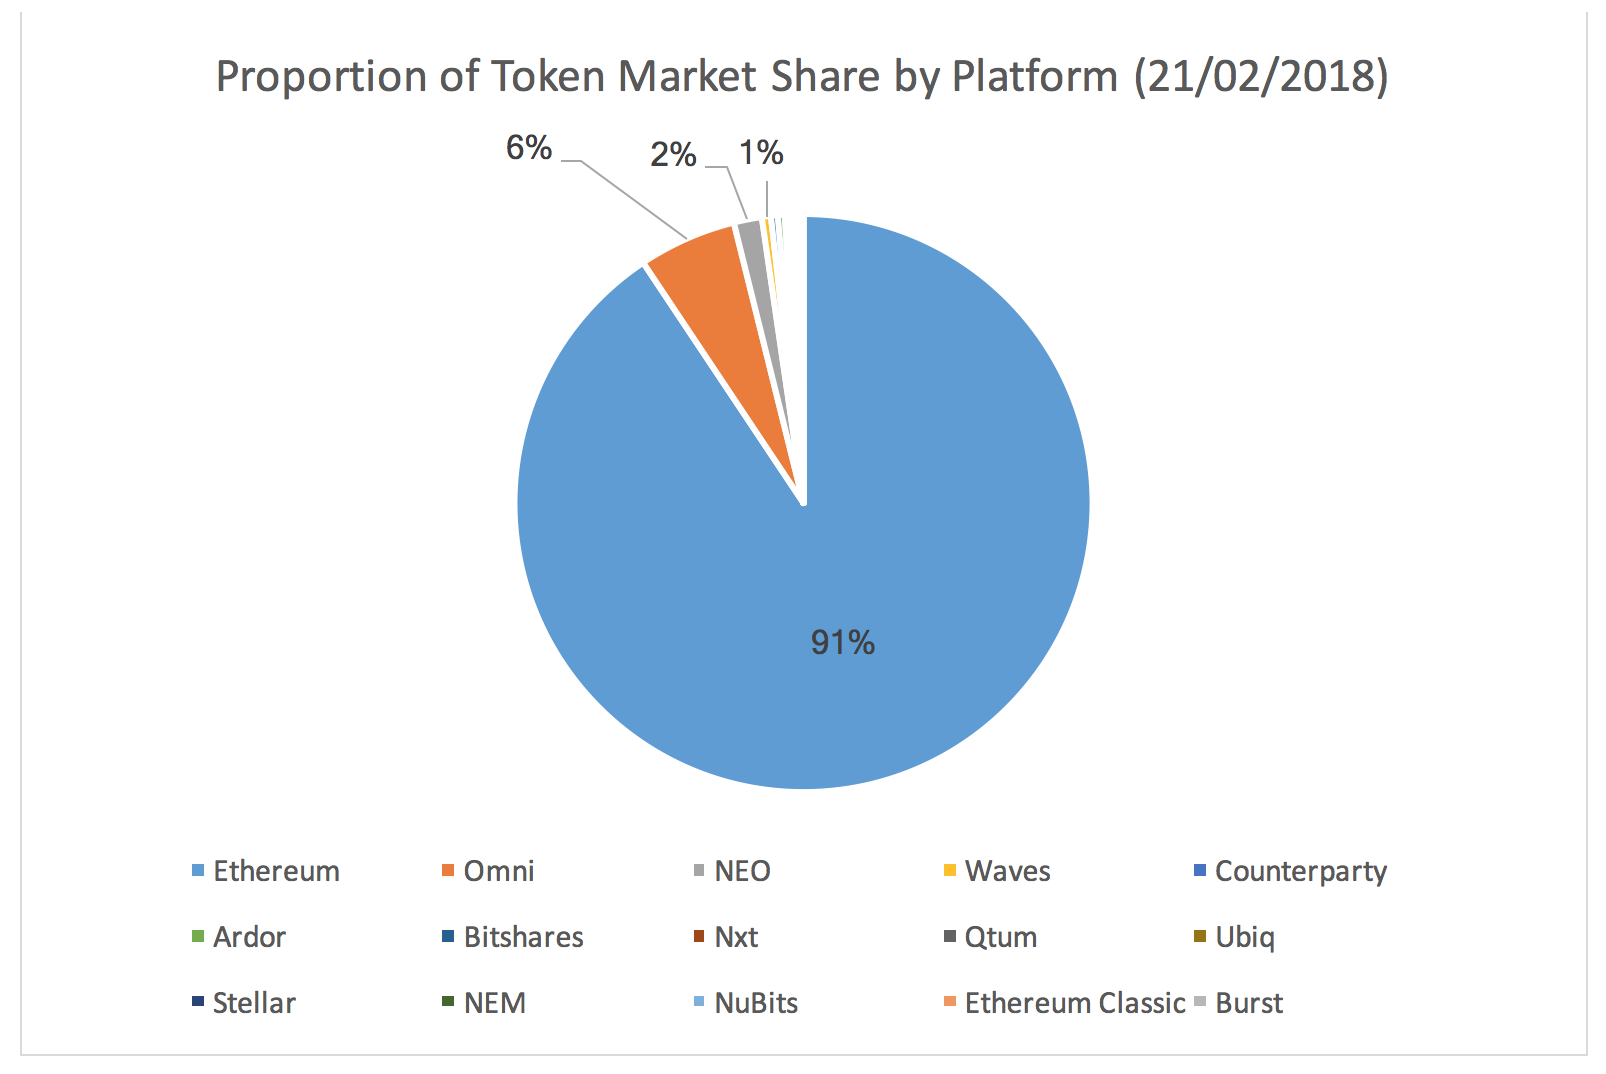
\includegraphics{~/Desktop/Everything/R/Working Directory/Cryptocurrency book/pictures/Token.png}
\caption{Ethereum host the vast majority of tokens}
\end{figure}

\subsection{Analysis of Top Ten Ethereum
Tokens}\label{analysis-of-top-ten-ethereum-tokens}

\begin{figure}[htbp]
\centering
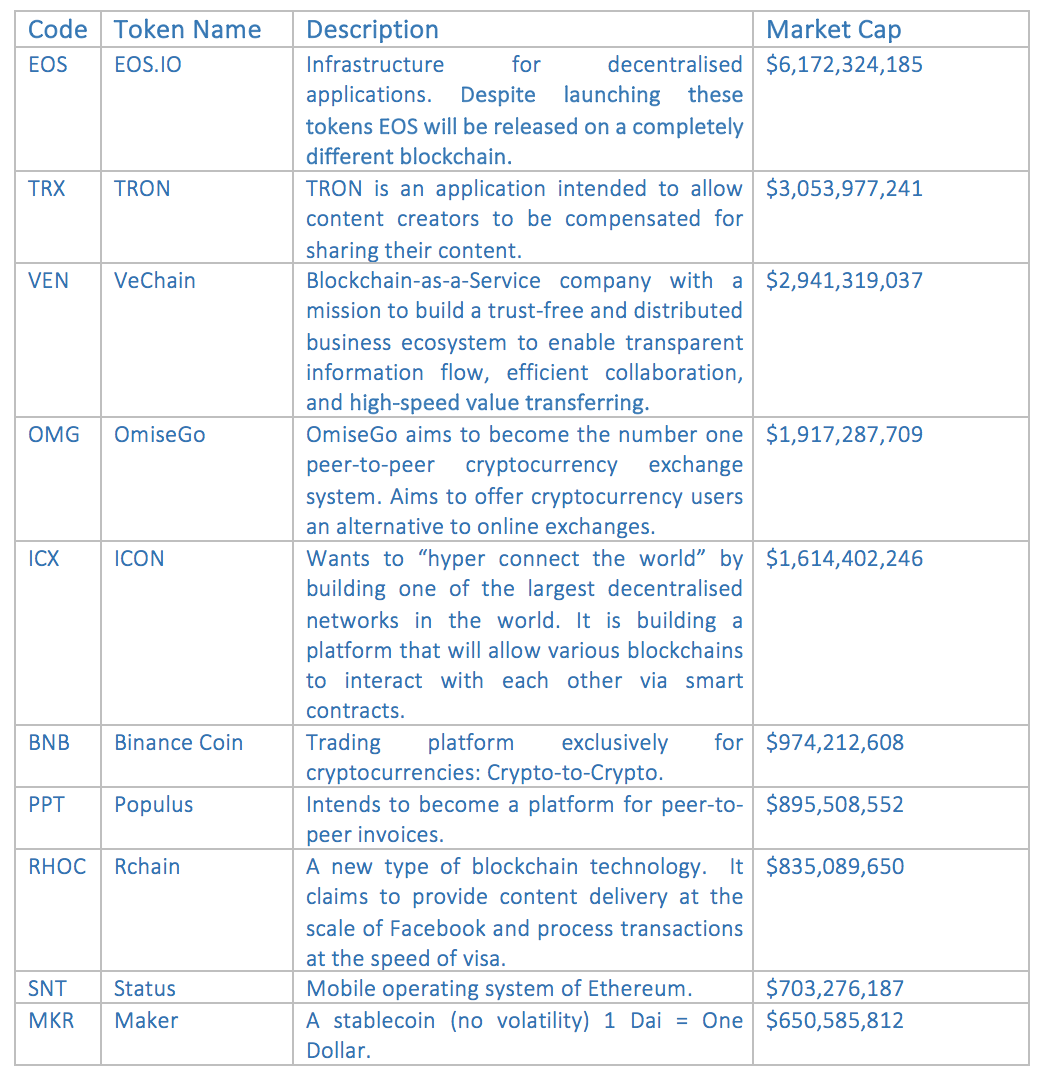
\includegraphics{~/Desktop/Everything/R/Working Directory/Cryptocurrency book/pictures/Tokens_built_on_ethereum.png}
\caption{Some of these tokens are considered valuable to appear on the
\url{http://www.coinmarketcap.com} top 20 list}
\end{figure}

\chapter{Additional data}\label{additional-data}

This is an R Markdown document. Markdown is a simple formatting syntax
for authoring HTML, PDF, and MS Word documents. For more details on
using R Markdown see \url{http://rmarkdown.rstudio.com}.

When you click the \textbf{Knit} button a document will be generated
that includes both content as well as the output of any embedded R code
chunks within the document. You can embed an R code chunk like this:

\begin{Shaded}
\begin{Highlighting}[]
\KeywordTok{summary}\NormalTok{(cars)}
\end{Highlighting}
\end{Shaded}

\begin{verbatim}
##      speed           dist       
##  Min.   : 4.0   Min.   :  2.00  
##  1st Qu.:12.0   1st Qu.: 26.00  
##  Median :15.0   Median : 36.00  
##  Mean   :15.4   Mean   : 42.98  
##  3rd Qu.:19.0   3rd Qu.: 56.00  
##  Max.   :25.0   Max.   :120.00
\end{verbatim}

\section{Including Plots}\label{including-plots}

You can also embed plots, for example:

\includegraphics{Cryptocurrency_Research_files/figure-latex/pressure-1.pdf}

Note that the \texttt{echo\ =\ FALSE} parameter was added to the code
chunk to prevent printing of the R code that generated the plot.

\bibliography{book.bib,packages.bib}


\end{document}
